\documentclass[oneside,12pt]{DISCSthesis}
\usepackage{graphicx}
\usepackage{longtable}
\usepackage{setspace}
\usepackage{soul}
\usepackage{amsmath}
\usepackage{algpseudocode}
	\renewcommand{\algorithmiccomment}[1]{\hskip0em$\triangleright$ \emph{#1}}
	\renewcommand{\algorithmicrequire}{\hspace*{6pt}\textbf{Input:}}
	\renewcommand{\algorithmicensure}{\hspace*{6pt}\textbf{Output:}}

%\documentclass{article}
\begin{document}
\ThesisAuthor{\textbf{Maria Clara Isabel D. Sia}}
\ThesisTitle{\textbf{Improving An Exact Solution to the ($l$, $d$)-Planted Motif Problem}}
\ThesisArea{Computer Science}
\ThesisDefenseYear{2015}
% \DefenseDate{10 July 2013}
% \ThesisGrade{}

\DepartmentHead{MARLENE M. DE LEON, Ph.D.}
\SchoolHead{EVANGELINE P. BAUTISTA, Ph.D.}
\ThesisAdviser{PROCESO L. FERNANDEZ, JR., Ph.D.}
\FirstPanelMember{XXX, Ph.D.}
\SecondPanelMember{XXX, Ph.D.}
\ThirdPanelMember{XXX, Ph.D.}

\ThesisStyle{MS}{Draft}{-10pt}{15pt}
% Choices for the 1st argument: MS, PhD
% Choices for the 2nd argument: Final, FinalWithCorner, Draft

\FrontMatter
% \input{acknowledgements}

\begin{abstract}
	DNA motif finding is widely recognized as a difficult problem in computational biology and computer science. Because of the usual large search space involved, exact solutions typically require a significant amount of execution time before discovering a motif of length $l$ that occurs in an input set $\{S_{1} ,...,S_{n}\}$ of sequences, allowing for at most $d$ substitutions. 

	This study implements a novel improvement to EMS-GT, a motif search algorithm which operates on a compact bit-based representation of the search space. The improvement takes advantage of distance-related patterns in the search space, in order to speed up the bulk bit-setting operations performed by the algorithm. A Java implementation
	% ---run on synthetic datasets for various challenge instances of the ($l,d$) planted motif problem---
	is shown to be highly competitive against PMS8 and qPMS9, two current state-of-the-art exact algorithms. EMS-GT works extremely well for problems involving short motifs, outperforming both competitors for challenge instances with ($l,d$) values (9,2), (11,3), (13,4) and (15,5), showing runtime reductions of 76\%, 81\%, 77\% and 37\% respectively for these instances, while ranking second to qPMS9 for challenge instance (17,6).
	\end{abstract}

\tableofcontents
\listoffigures
\listoftables

\MainMatter

\chapter{Introduction}
	%section{Start of the intro}
		DNA motif finding is widely recognized as a difficult problem in computational biology and computer science. Motifs are sequences that occur repeatedly in DNA and have some biological significance \cite{das2007survey}; a motif might be a transcription factor binding site, a promoter element, a splicing site, or a marker useful for classification. There are many variants of motif finding problem in the literature. Some look for a motif that repeatedly occurs in a single sequence. Others look for a motif that occurs over some or all of a set of DNA sequences \cite{dasari2010efficient}. One of the latter type is the planted motif problem.\newline

		\begin{figure}[h] \label{fig:example}
			\centering
			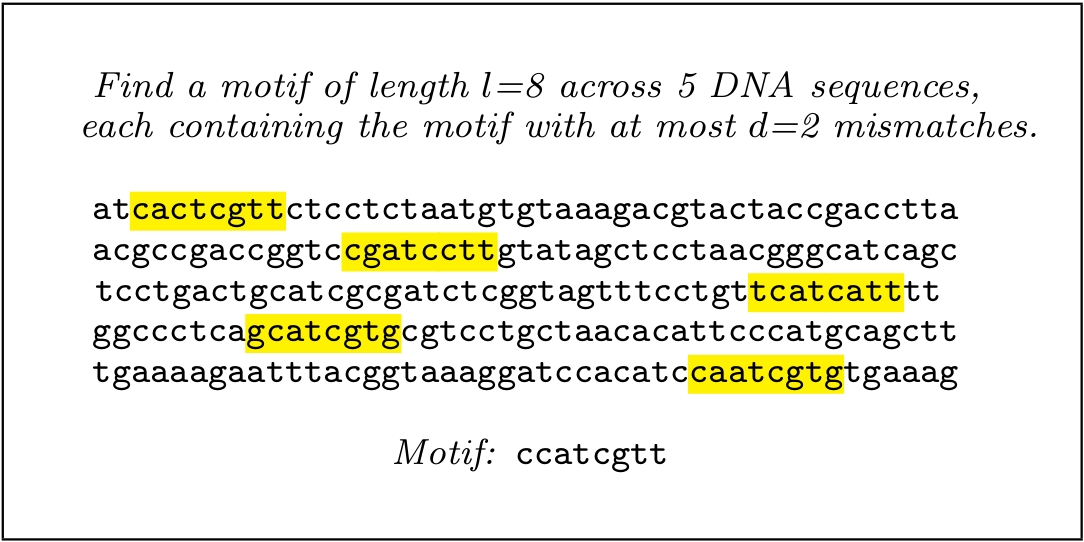
\includegraphics[width=5.5in]{img/example}
			\caption{Sample instance of the planted motif problem.}
			\end{figure}

		The planted motif problem simply asks: ``\emph{Given a set of DNA sequences, can we find an unknown motif of length $l$ that appears at different positions in each of the sequences} \cite{pevzner2000combinatorial}?'' Initially it seems an exhaustive string search will suffice for this problem. However, due to biological mutation, motif occurrences in DNA are allowed to differ from the original motif by up to $d$ characters. This greatly impacts complexity: two distinct variants of a motif---both counting as valid occurrences of the motif---might differ in as many as 2$d$ characters! Brute-force solutions quickly become infeasible as values of $l$ and $d$ increase. All of this shows why ($l$, $d$)-motifs are sometimes called ``subtle'' signals in DNA  \cite{pevzner2000combinatorial}, and why finding them is difficult and computationally expensive. In fact, the motif finding problem has already been shown to be NP-complete \cite{pms2014}. 

		This study is concerned with the EMS-GT (\emph{Exact Motif Search - Generate and Test}) algorithm \cite{nabos2015dissertation}, which solves the planted motif problem for any arbitrary instance up to $l$=17. This study investigates certain Hamming distance-related patterns appearing in EMS-GT's bit-based representation of the motif search space, and uses these to develop a novel speedup technique for EMS-GT.

	\section{Context of the Study}
		This section formally defines the planted motif problem. It also defines key terms used throughout this paper in discussing exact motif-search algorithms.

		\noindent\textbf{\boldmath DEFINITION 1. $l$-mer, Hamming distance, $d$-neighborhood}

		\noindent An \textbf{\boldmath $l$-mer} is a sequence of length $l$. Given a sequence $S$ of length $L > l$, the $i^{th}$ $l$-mer in $S$ starts at the $i^{th}$ position. The \textbf{\boldmath Hamming distance $dH$} between two $l$-mers of equal length is the number of characters that differ between them. ``Distance'' refers to Hamming distance in this paper, unless otherwise stated.
		\newline\hspace*{35pt} Ex. If $l$ = 5, the second $l$-mer in \texttt{gattaca} is \texttt{attac}.
		\newline\hspace*{55pt} $dH(\texttt{gattaca}, \texttt{cgttaga}) = 3$.

		\noindent The \textbf{\boldmath $d$-neighborhood of an $l$-mer $x$} is the set {\boldmath $N(x, d)$} of all $d$-neighbors of $x$: all $l$-mers $x'$ whose Hamming distance from $x$ is at most $d$, i.e., {\boldmath $dH (x, x') \leq d$}. 
		Meanwhile, the \textbf{\boldmath $d$-neighborhood of a sequence $S$} of length $L > l$ is the set {\boldmath $\mathcal{N}(S, d)$} of all $d$-neighbors of all the $l$-mers in $S$.
		\newline\hspace*{35pt} Ex. \texttt{gatct}, \texttt{cctta}, and \texttt{aatta} are all in $N(\texttt{gatta}, 2)$.
		\newline\hspace*{55pt} For $l$ = 5,
			$\mathcal{N}(\texttt{gattaca}, 2) 
					= N(\texttt{gatta}, 2) \cup 
						N(\texttt{attac}, 2) \cup
						N(\texttt{ttaca}, 2)$.\newline
		
		\noindent\textbf{\boldmath DEFINITION 2. ($l,d$) Planted Motif Problem}
		\newline We formally define the ($l$,$d$) planted motif problem as follows:\bigskip

		\noindent\hspace*{50pt} Given a set $\mathcal{S} = \{S_{1},...S_{t}\}$ of $n$ DNA sequences of length $L$,
		% \newline \hspace*{52pt} the motif length $l$, and the number of allowable mismatches $d$,
		\newline \hspace*{50pt} find $M$, the set of sequences (or motifs) of length $l < L$
		\newline \hspace*{50pt} which have at least one $d$-neighbor in each sequence in $S$. %in $S$.
		
	\section{Objectives of the Study}
		The main objective of this study is to improve the performance of the EMS-GT algorithm. Specifically, it aims:
		\begin{enumerate}
		\item To develop a speedup technique for EMS-GT that takes advantage of distance-related patterns in the motif search space.
		\item To evaluate the resulting technique with regard to improvement in runtime and solvable problem instances.
		\item To evaluate the improved version of EMS-GT against state-of-the-art motif search algorithms.
		\end{enumerate}

	\section{Research Questions}
		This study aims to answer the question: How can the performance of the EMS-GT algorithm be improved?
		Specifically, it aims to answer the following:

		\begin{enumerate}
		\item How can distance-related patterns observed within the motif search space be exploited in a speedup technique for EMS-GT?
		\item What performance improvement does a pattern-based speedup technique, with regard to runtime and solvable problem instances?
		\item How does the improved version of EMS-GT compare with state-of-the-art motif search algorithms?
		\end{enumerate}

	\section{Significance of the Study}
		Motif finding in DNA and other types of nucleotide sequences is an important task in bioinformatics. Genome analysis requires fast, efficient algorithms to identify biological motifs which may be linked to protein synthesis, gene function, or even disease and targets for medical treatment. 

		Improvinging the EMS-GT algorithm, which was shown to be competitive with the state-of-the-art, results in an even faster option for real-world motif finding applications. Furthermore, this study's investigation and insights regarding distance-related patterns within an organized search space may prove applicable to other types of search tasks, pattern-matching tasks, and problems involving Hamming distances.

	\section{Scope and Limitations of the Study}
		This study is concerned with integrating a novel bit-masking speedup technique into the existing Java implementation of EMS-GT. The improved version is benchmarked by its runtime on synthetic datasets for challenging instances of the problem. (EMS-GT had been previously tested for correctness using real biological data with known motifs; re-testing would be redundant since the speedup technique does not change the logic of the algorithm.)	
		Furthermore, the performance of EMS-GT is compared to that of PMS8 and qPMS9 running on a single core. Although both competitor algorithms are also capable of using multiple procesors, parallelization is beyond the current scope of the speedup techniques explored for EMS-GT.

\chapter{Review of Related Literature}
	Motif finding is a well-studied problem in computing. Various motif search algorithms have been developed,
	falling into two categories: \emph{heuristic} and \emph{exact}. This section gives an overview of algorithms
	of both types, and provides an in-depth description of the exact algorithm EMS-GT.
	
	\section{Heuristic Algorithms}
		Heuristic algorithms perform an iterative local search, for instance by repeatedly refining an input sampling or projection until 
		a motif is found. 

		Gibbs sampling \cite{lawrence1993detecting} and Expectation Maximization (EM), used in the motif-finding tool MEME \cite{lawrence1990expectation,bailey1995unsupervised} both use probabilistic computations to improve an initial random alignment. (An alignment is simply a vector $(a_{1}, a_{2},...,a_{n})$ of $n$ positions, which predicts that the motif occurs at position $a_{i}$ in the given sequence $S_{i}$.) Gibbs sampling attempts to refine the alignment one position at a time; %in contrast,
		EM may recompute the entire alignment in a single iteration. 

		Projection \cite{blanchette2002discovery} combines a pattern-based approach with EM's probabilistic approach, trying to guess every successive character of a tentative motif and using EM to verify its guesses. GARPS \cite{huo2009combining} uses a random version of the projection strategy, in tandem with the iteratively self-correcting Genetic Algorithm (GA), for yet another iterative approach. These are just some of many successful heuristic algorithms for motif finding.

	\section{Exact Algorithms}
		While they can be efficient, heuristic approaches are non-exhaustive and thus not always guaranteed to find a solution. Exact motif search algorithms, on the other hand, perform an exhaustive search of possible motifs and so always find the planted motif.

		WINNOWER \cite{pevzner2000combinatorial} and its successor MITRA \cite{eskin2002finding} are exact algorithms that look at pairwise $l$-mer similarity to find motifs. In a set of DNA sequences, there are numerous pairs of ``similar'' $l$-mers, which come from different sequences and have Hamming distances of at most 2$d$ from each other (meaning that they could possibly be two $d$-neighbors of the same $l$-mer). WINNOWER represents these pairs in a graph, with $l$-mers as nodes and edges connecting $l$-mer pairs. It then prunes the graph to identify ``cliques'' of pairs that indicate a motif. MITRA refines this graph representation into a mismatch tree containing all possible $l$-mers, organized by prefix. The tree structure allows MITRA to eliminate entire branches at a time, making it significantly faster than WINNOWER at removing the many spurious edges that are not part of any motif clique.

		The BitBased algorithm \cite{dasari2010efficient} uses approaches that are similar to EMS-GT's (see subsection 2.3.1): it maps $l$-mers to binary strings of length $2l$, and represents the motif search space with an array of bits. The main difference is that BitBased is optimized for parallel computation on multiple cores, requiring specialized GPU hardware (Nvidia Tesla C1060 or S1070). BitBased is able to solve the challenge problem instance (21,8) in 1.1 hours.

	\subsection{PMS8 and qPMS9}
		The current state-of-the-art exact algorithms are PMS8 and qPMS9, from the Panoptic Motif Search (PMS) series
		 developed by Rajasekaran et al
		\cite{pms2007,pms2014,pms2015}. The idea in both PMS8 and qPMS9 is to form all possible tuples of $n'$ ``similar'' $l$-mers, for some $n' < n$, and then determine whether the common neighbors of $l$-mers in these tuples are motifs. This approach proceeds in two main steps:

		\begin{enumerate}
			\item {\em Sample-driven step}\newline
			This step chooses a tuple $T$ of $n'$ ``similar'' $l$-mers from $n'$ distinct DNA sequences in the set $\mathcal{S}$. Similarity means that the $l$-mers in the tuple have a common neighbor; this implies that the distance between any two $l$-mers in $T$ must be less than $2d$.
			%To build $T$, the algorithm repeatedly chooses an $l$-mer from a different sequence each time, avoiding $l$-mers with distances over $2d$ from any of the $l$-mers already in $T$. This ensures that new $l$-mers have neighbors in common with the others.
			\begin{equation} T = \{l_{1}, l_{2}, ..., l_{n'}\},\ \ \ \ \ \ 
			dH(l_{i}, l_{j}) \leq 2d\ \ \forall\ l_{i}, l_{j} \in T \end{equation}

			\item {\em Pattern-driven step}\newline
			This step intersects the $d$-neighborhoods of $l_{1}, l_{2}, ..., l_{n'}$ to form the set $C$ of their common neighbors. It then checks each $l$-mer $c$ in $C$, to determine whether a $d$-neighbor of $c$ appears in all of the $n-n'$ remaining sequences (i.e., those sequences which did not initially contribute an $l$-mer to $T$). If this is the case, $c$ is accepted as a motif.
			\begin{equation} C = N(l_{1}, d) \cap N(l_{2}, d) \cap...\cap N(l_{n'}, d). \end{equation}
		\end{enumerate}
		\vspace{-5mm}
		\noindent Exhaustively building all ``similar'' $n'$-tuples requires significant runtime and many false starts (i.e., the algorithm has built a tuple to size $m < n'$, only to find that no further similar $l$-mers can be found).
		PMS8 reduces this by improving the search for additional $l$-mers, using stricter pruning conditions for similarity % ---the presence of common neighbors---
		between {\em three} $l$-mers (two from the tuple, and the one to be added). This method of testing similarity for $l$-mer triples, instead of pairs, quickly recognizes and discards false starts. For even greater efficiency, qPMS9 intelligently prioritizes adding $l$-mers that are highly distant from those already in the tuple, such that common neighborhood becomes smaller and faster to check through.
		In practice, both PMS8 and qPMS9 have been implemented to run on multiple processors with the OpenMPI C library, allowing them to solve highly challenging problem instances with ($l, d$) as large as (50, 21) in a few hours.

	\newpage
	\section{EMS-GT}
		EMS-GT, first developed by Nabos \cite{nabos2015dissertation}, is an exact motif search algorithm based on the candidate generate-and-test principle.
		It operates on a compact bit-based representation of the search space.
		% , identifying the common $d$-neighbors of the $n$ given DNA sequences as motifs. 
		Similar to PMS8 and qPMS9, the main idea of EMS-GT is to narrow down the search space to a small set of ``candidate'' motifs based on the first $n'$ sequences, then to do a brute-force search for neighbors of each candidate in the remaining $(n - n')$ sequences to confirm whether or not the candidate is a motif.
		EMS-GT's approach proceeds in two main steps:
		\begin{enumerate} %[label={\em (\alph*)}]
			\item {\em Generate candidates}\newline
			This step intersects the $d$-neighborhoods of the first $n'$ sequences $S_{1},S_{2},...,S_{n'}$. Every $l$-mer in the resulting set $C$ is a candidate motif.
				\begin{equation} C = \mathcal{N}(S_{1}, d) \cap \mathcal{N}(S_{2}, d) \cap...\cap \mathcal{N}(S_{n'}, d). \end{equation}
			\item {\em Test candidates}\newline
			This step simply checks each candidate motif $c$ in $C$, to determine whether a $d$-neighbor of $c$ appears in all of the remaining sequences $S_{n'+1},S_{n'+2},...,S_{n}$. If this is the case, $c$ is accepted as a motif in set $M$.
				\begin{equation} M = C \cap \mathcal{N}(S_{n'+1}, d) \cap...\cap \mathcal{N}(S_{n}, d). \end{equation}
			\end{enumerate}

		\newpage{\setstretch{1.0}
		\noindent\hspace*{6pt}{\bf Algorithm 2.1} \textsc{Exact Motif Search - Generate and Test}\small
		\begin{algorithmic}[1] \label{alg:EMS-GT}
			\Require set $S = \{S_{1},S_{2},...,S_{n}\}$ of $L$-length sequences, \newline \hspace*{25pt}motif length $l$, allowable mismatches $d$
			\Ensure set $M$ of candidate motifs %\vspace*{6pt}
			% \State 
			\State $C \leftarrow \{\}$										\hspace*{200pt}\Comment{generate candidates}
			\State $\mathcal{N}(S_{1},d) \leftarrow \{\}$
			\For{$j \leftarrow 1$ to $L-l+1$}
				\State $x \leftarrow j^{th} l$-mer in $S_{1}$
				\State $\mathcal{N}(S_{1},d) \leftarrow \mathcal{N}(S_{1},d) \cup N(x,d)$
			\EndFor
			\State $C \leftarrow \mathcal{N}(S_{1},d)$
			\For{$i \leftarrow 2$ to $n'$}
				\State $\mathcal{N}(S_{i}, d) \leftarrow \{\}$
				\For{$j \leftarrow 1$ to $L-l+1$}
					\State $x \leftarrow j^{th} l$-mer in $S_{1}$
					\State $\mathcal{N}(S_{i},d) \leftarrow \mathcal{N}(S_{i},d) \cup N(x,d)$
				\EndFor
				\State $C \leftarrow C \cap \mathcal{N}(S_{i},d)$
			\EndFor
			\State $M \leftarrow \{\}$										\hspace*{200pt}\Comment{test candidates}
			\For{each $l$-mer $u$ in $C$}
				\State $isMotif \leftarrow$ true
				\For{$i \leftarrow (n'+1)$ to $n$}
					\State $found \leftarrow$ false
					\For{$j \leftarrow 1$ to $L-l+1$}
						\State $x \leftarrow j^{th} l-$mer in $S_{i}$
						\If{$dH(x,u) \leq d$}
							\State $found \leftarrow$ true
							\State break
						\EndIf
					\EndFor
					\If{!$found$}
						\State $isMotif \leftarrow$ false
						\State break
					\EndIf
				\EndFor
				\If{$isMotif$}
					\State $M \leftarrow M \cup u$
				\EndIf
			\EndFor
			\State\Return $M$
			\end{algorithmic}
		}


		\noindent In practice, EMS-GT must perform speedy operations on an array of bits representing the entire motif search space. Subsections 2.3.1 to 2.3.4 discuss the efficiency strategies EMS-GT uses for important tasks such as representing sets in the search space, determining whether $l$-mers are neighbors, and generating all possible $d$-neighbors of a given $l$-mer.

		\subsection{Bit-based set representation and $l$-mer enumeration}
			The motif search space consists of the $4^{l}$ possible $l$-mers that can be formed from the nucleic alphabet \{\texttt{a}, \texttt{g}, \texttt{c}, \texttt{t}\}. To efficiently represent sets---such as a $d$-neighborhood, or a set of candidate motifs---within this space, EMS-GT assigns each of the $4^{l}$ $l$-mers a bit flag in an array, set to 1 if the $l$-mer is a member of the set and 0 otherwise. Bit flags correspond to $l$-mers via a simple mapping: EMS-GT maps an $l$-mer $s$ to a bit flag index $x$ by replacing each character with 2 bits (\texttt{a=00}, \texttt{c=01}, \texttt{g=10}, \texttt{t=11}). Note that this mapping scheme enumerates $l$-mers in strict alphabetical order.

			\noindent \hspace*{40pt}{\small Ex. \texttt{tacgt} maps to \texttt{1100011011} = 795; thus, its flag is the $795^{th}$ bit in the array.
				% \hspace*{58pt} Thus, the flag for \texttt{tagct} is bit 795 in the array.}

		\subsection{Bit-array compression}
			EMS-GT's implementation compresses the required set-representation array of $4^{l}$ bits into an equivalent array of $\frac{4^{l}}{32}$ 32-bit integers. The $x^{th}$ bit is now found at position ($x$ mod 32) of the integer at array index $\frac{x}{3}$.\newline
			\hspace*{40pt}{\small Ex. \texttt{tacgt} maps to \texttt{1100011011} = 795 in decimal.\newline
				\hspace*{58pt} \emph{array index}  = $\frac{795}{32}$ = 24 , \hspace*{5pt} \emph{bit position} = 795 mod 32 = 27;\newline %\newline\hspace*{58pt} 
				\hspace*{58pt}Thus, the flag for \texttt{tacgt} is the 27$^{th}$ bit of the integer at array index 24.}
			% \begin{figure}[h] \label{fig:bitarray_demo}
			% 	\end{figure}

		\subsection{XOR-based Hamming distance computation}
			The mapping of $l$-mers to binary numbers  is also useful for computing Hamming distances. An exclusive OR (XOR) bitwise operation between the mappings of two $l$-mers will produce a nonzero pair of bits at every mismatch position; counting these nonzero pairs of bits in the XOR result gives us the Hamming distance. See Algorithm 2.2 for the implementation.\newline
			\noindent\hspace*{40pt} {\small Ex.	\texttt{tacgt} maps to \texttt{1100011011} \newline
				\vspace*{2pt}\hspace*{62pt} \texttt{ttcgg} maps to \texttt{1111011010} \newline				
				\hspace*{62pt}	XOR produces \hspace*{3pt}\texttt{00\hl{11}0000\hl{01}} = 2 mismatches.}

		\subsection{Recursive neighborhood generation}
			To generate a $d$-neighbor of an $l$-mer $x$, we choose $d' \leq d$ positions from 1, 2,..., $l$-1, $l$ and change the character at each of the $d'$ positions in $x$. EMS-GT uses a recursive procedure (Algorithm 2.3) to do this, effectively (1) traversing the tree of all $d$-neighbors and (2) setting the bit flag in the neighborhood array $N$ for each neighbor it encounters. Since we choose up to $d$ positions in the $l$-mer, and have 3 possible substitute characters at each position, the size of the neighborhood $N(x,d)$ is given by: %\bigskip \hspace*{20pt}
			\begin{equation}
				|N(x,d)| = \sum_{i=0}^d \binom{l}{i} 3^{i}
			\end{equation}

		\newpage
		{\setstretch{1.0}
			\noindent \hspace*{6pt}{\bf Algorithm 2.2} \textsc{Hamming distance computation}\small
			\begin{algorithmic}[1]\label{alg:hamming-distance-comp}
				\Require $l$-mer mappings $u$ and $v$
				\Ensure $dH(u,v)$\vspace*{6pt}

				\State $dH(u,v) = 0$
				\State $z \leftarrow u ^ v$
				\For {$i \leftarrow 1$ to $l$}
				\If{$z$ \& 3 != 0}
				\State $dH(u,v) \leftarrow dH(u,v) + 1$
				\EndIf
				\State $z \leftarrow z >>$ 2
				\EndFor
				\State\Return $dH(u,v)$
				\end{algorithmic}
			}

			\bigskip\bigskip\bigskip

		{\setstretch{1.0}
			\noindent \hspace*{6pt}{\bf Algorithm 2.3} \textsc{Recursive neighborhood generation}\small
			\begin{algorithmic}[1]
				\label{alg:recursive-nbr-gen}
				\Require DNA sequence $S$, motif length $l$, mismatches $d$
				\Ensure bit-array $\mathcal{N}$ representing $\mathcal{N}(S,d)$ \vspace*{6pt}
				% \For{$i \leftarrow$ 1 to $4^{l}$}
				\State $\mathcal{N}[lmer] \leftarrow 0,\ \ \forall\ lmer \in $ search space 
				% \EndFor
				\For{each $l$-mer $x$ in $S$}
				\State \textsc{AddNeighbors}($x$, 0, $d$) \hspace*{79pt}\Comment{recursive procedure}
				\EndFor
				\newline
				\State \Comment{make $d$ changes in $l$-mer $x$, from position $s$ onward}
				\Procedure{AddNeighbors}{$x$, $s$, $d$}
					\For{$i \leftarrow s$ to $l$}
						\State $\Sigma' \leftarrow$ \{\texttt{a}, \texttt{g}, \texttt{c}, \texttt{t}\} $- x_{i}$ \hspace*{79pt}\Comment{\small remove $i^{th}$ character of $x$}
						\For{$j \leftarrow 1$ to $|\Sigma'|$}
							\State $neighbor \leftarrow concatenate(x_{1...i-1},\Sigma_{j},x_{i+1...l})$
							\State $\mathcal{N}[neighbor] \leftarrow 1$
							\If{$d > 1$ and $i < l$}
								\State \textsc{AddNeighbors}($neighbor$, $i+1$, $d-1$)
							\EndIf
						\EndFor
					\EndFor
				\EndProcedure
				\State\Return $\mathcal{N}$
				\end{algorithmic}
			}

\chapter{Methodology}
	This section briefly describes how a novel speedup technique for EMS-GT was explored and implemented.
	It then describes the procedure for evaluating the improved version of the EMS-GT algorithm.

	\section{Improving EMS-GT}
		The Java implementation of EMS-GT operates on a compact, bit-based enumerative representation of the motif search space. Since a significant part of runtime is spent finding and setting bits in this bit-based representation, speedup techniques were explored for the bit-setting portion of the algorithm.

		Snapshots of EMS-GT's main data structure (an array of $4^l$ bit flags representing the entire search space) were taken at various times during program execution, and examined for features that might allow for a more efficient algorithm. It became clear that $l$-mer neighborhoods, when represented in this data structure, were made up of repeating block patterns; we examined the underlying distribution of Hamming distances in these blocks to explain the patterns.

		By finding connections to (1) EMS-GT's alphabetical $l$-mer enumeration scheme and (2) the additive property of Hamming distances, we were able to justify the original observation, which was: ``A bit-array $N$ representing the neighborhood $N(x,d)$ can be divided into consecutive blocks of $4^k$ bits each, where each block will conform to one of at most ($k+2$) patterns.'' The full explanation of block patterns in $N$ is written out in Section 4.1.
		
		Working forwards, we then developed a procedure which can quickly build any neighborhood $N$ in blocks, referring to a pre-generated lookup table of the possible block patterns. This technique was integrated into the Java implementation of EMS-GT.

	\section{Evaluation}
		The improved version of EMS-GT was compared to the original EMS-GT algorithm, as well as to the state-of-the-art algorithms PMS8 and qPMS9, by benchmarking their performance on challenging instances of the ($l, d$) planted motif problem. An ($l$, $d$) problem instance is defined to be a challenging instance if $d$ is the largest value for which the expected number of $l$-length motifs that would occur in the input by random chance does not exceed some limit---typically 500 random motifs \cite{pms2015}. The specific challenge instances used were (9,2), (11,3), (13,4), (15,5), and (17,6), as identified in \cite{pms2015,pms2007}. 

		\subsection{Synthetic Datasets}
			Synthetic datasets were created using a DNA sequence generator written in Java. Each nucleotide character in a sequence is randomly generated; \{\texttt{a}, \texttt{g}, \texttt{c}, \texttt{t}\} each have a 25\% chance of being selected, independent from other characters in the sequence.
			The motif is then planted at a random position in the sequence. As prescribed in \cite{pevzner2000combinatorial} every dataset contains 20 DNA sequences each 600 bases long, with an ($l$, $d$) motif planted exactly once in each sequence.

\chapter{Results and Analysis}
	This section provides a step-by-step derivation of the distance-related patterns that occur within a bit-array representing an $l$-mer neighborhood in EMS-GT. It then describes how a speedup technique for EMS-GT based on these patterns was implemented. Finally, it quantifies the performance improvement due to this technique.
	
	\section{\boldmath Deriving distance-related patterns in $l$-mer neighborhoods}
		\begin{enumerate}
			\item We can represent the neighborhood $N(x,d)$ of an $l$-mer $x$ as an array $N$ of $4^{l}$ bit flags, set to 1 if the corresponding $l$-mer is a neighbor and 0 otherwise.
				\begin{equation}
					N_{x'} = \left\{
					\begin{array}{rl}
						1 & \text{if } dH(x,x') \leq d,\\
						0 & \text{otherwise.}%\text{if } dH(x,x') > d.
					\end{array} \right.
					\text{ for any $l$-mer }x'.
					\end{equation}

			\item We find that if we divide this bit-array $N$ into consecutive blocks of $4^{k}$ flags each, for some {\b\boldmath block degree $k$}, $0 < k < l$, each block will conform to one of at most ($k + 2$) possible bit patterns. We exploit this regularity to build $N$ in blocks.

			\item Say we wish to generate $N(x,d)$ for some $l$-mer $x$. We divide $x$ into its {\bf\boldmath prefix $y$ }(first $l - k$ characters) and its {\bf\boldmath $k$-suffix $z$} (last $k$ characters).

				{\small\hspace*{40pt}Ex. For $k$ = 5,\ \ $x$ = \texttt{acgtacgtacgt} $\rightarrow$ \ \ $y$ = \texttt{acgtacg} and $z$ = \texttt{tacgt}.}

			As later explained in steps 7-8, the prefix will decide which of ($k + 2$) patterns is applicable in a particular block in $N$, while the $k$-suffix will determine the structure of these ($k + 2$) patterns.

			\item We generate the distribution $D(z)$ of Hamming distances from $z$ to all $4^{k}$ possible $k$-suffixes. We consider this distribution to be ``centered'' at $z$.

				\begin{figure}[h] \label{fig:D_tacgt}
					\
					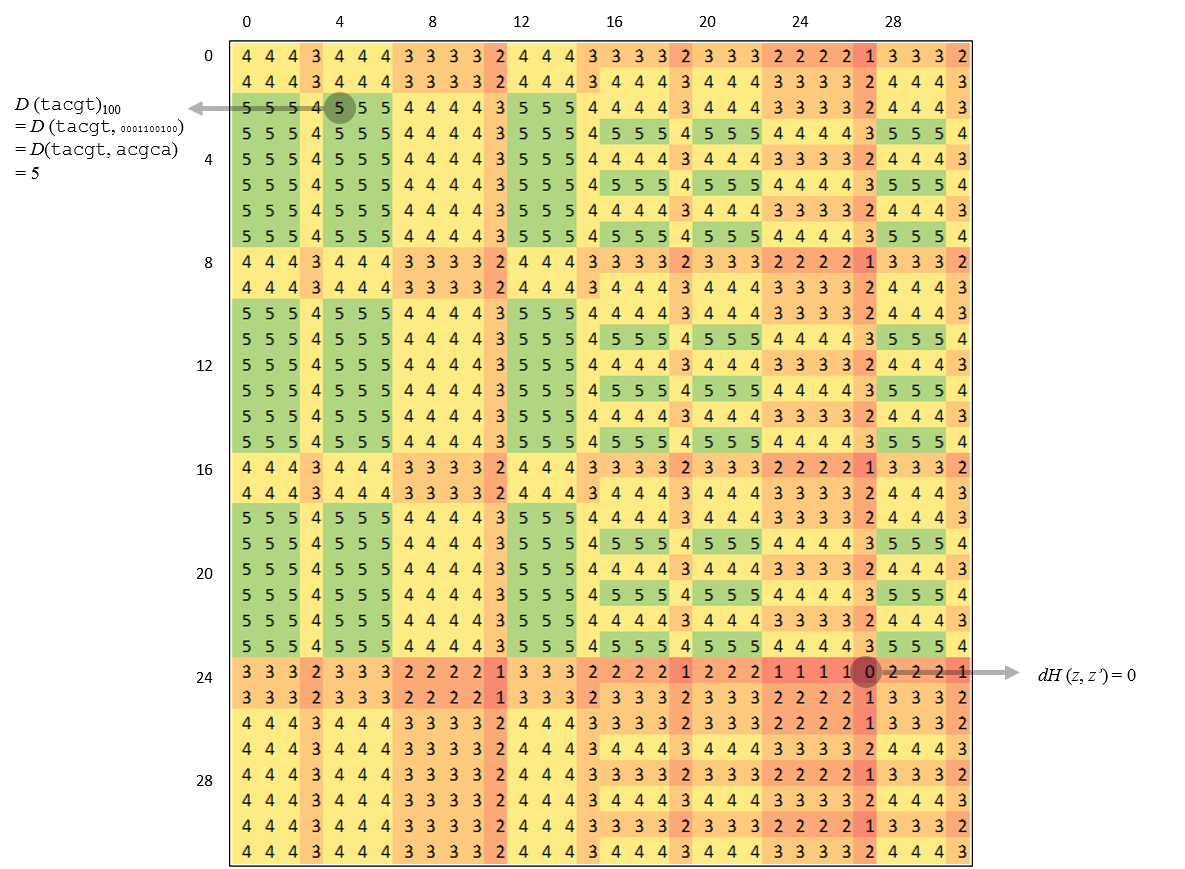
\includegraphics[width=6.0in]{img/D(tacgt)_marked_2}
					\caption{Distance distribution from \texttt{tacgt} to all $4^{5} = 32 \times 32$ $k$-suffixes, $k$=5.}
					\end{figure}

			The value in the $p^{th}$ cell---found at row $\frac{p}{32}$, column $p\ \emph{mod}\ 32$---of the $32 \times 32$ table in Figure 4.\ref{fig:D_tacgt} is the distance $dH (z, z’)$ from $z$ = \texttt{tacgt} to the $k$-suffix $z'$ which maps to the binary number $p$.

				{\small\hspace*{40pt}Ex. $D(\texttt{tacgt})_{100}$\ \ \ \ \ = $dH(\texttt{tacgt}, \texttt{0b0001100100})$
				\newline\hspace*{137pt} = $dH(\texttt{tacgt}, \texttt{acgca})$
				\newline\hspace*{137pt} = 5 ,\ \ \ \ at row $\frac{100}{32} = 3$, column $(100\ \emph{mod}\ 32) = 4$
				}\newline

			\item Due to the alphabetical enumeration, the $4^k\ l-$mers grouped together in a block will all begin with the same ($l - k$) characters, which we will call the {\bf\boldmath block prefix $y'$}. We can compute a single prefix distance $d_{y'}$ for an entire block: this is simply the distance $dH(y, y')$ between $x$'s prefix and the block prefix.

				{\small\hspace*{40pt} Ex.\ \ \ \ For the block containing $l$-mers \{\texttt{acgttgcaaaaa} to \texttt{acgttgcttttt}\},
				\newline\hspace*{70pt} the prefix distance from $z$ = \texttt{acgtacgtacgt} is 
				\newline\hspace*{70pt} $d_{y'} = dH(\texttt{acgtacg}, \texttt{acgttgc}) = 3.$
				}

			\item We can infer that the distance between any two $l$-mers is equal to the sum of the distance between their prefixes and the distance between their $k$-suffixes %(in other words, Hamming distances are additive);
			; thus, knowing $d_{y'}$ and $\mathcal{D}(z)$ for some $l$-mer $x' = y'z'$ in the search space, we can compute its distance from $x$ as:
				\begin{equation}
					dH(x,x') = d_{y'} + \mathcal{D}(z)_{z'}
					\end{equation}

			\item With Equations (4.1) and (4.2), we can redefine the criteria for setting a bit in $N$:
				\begin{equation}
					N_{x'} = \left\{
					\begin{array}{rl}
						1 & \text{if } d_{y'} + \mathcal{D}(z)_{z'} \leq d,\\
						0 & \text{otherwise.}%\text{if } d_{y'} + \mathcal{D}(z)_{z'} > d.
					\end{array} \right.
					\text{ for }x' = y'z'.
					\end{equation}
				From this we see that a bit at position $z'$ within a block with prefix $y'$ will be set if and only if $D(z)_{z'} \leq d-d_{y'}$. The values in $D(z)$ range from 0 to $k$; therefore, we examine ($k + 2$) cases for the value of ($d - d_{y'}$) with respect to the range (0, ..., $k$):

					{\small
					\hspace*{40pt}{\bf\boldmath Case $-1$:}
					\hspace*{54pt} $d-d_{y'} < 0$, \hspace*{24pt}no bits in the block are set;\newline
					\hspace*{40pt}{\bf\boldmath Case 0:}
					\hspace*{66pt} $d-d_{y'} = 0$, \hspace*{24pt}the ``center'' bit (at position $z$) is set;\newline
					\hspace*{40pt}{\bf\boldmath\boldmath Cases 1 to $k-1$:}
					\hspace*{11.5pt} $1 \leq d-d_{y'} < k$, \hspace*{5pt}some of the bits are set; and\newline
					\hspace*{40pt}{\bf\boldmath Case $k$:}
					\hspace*{66pt}$d-d_{y'} \geq k$, \hspace*{24pt}all bits in the block are set.}

			\item We see that the ($k + 2$) patterns of blocks in $N$ correspond to the ($k + 2$) cases listed in step 7, and thus the pattern to be used in a certain block is indicated by the value of ($d - d_{y'}$). Meanwhile, the polarity (0 or 1) of a bit in one of these patterns is determined by the value of $D(z)$ at the corresponding position.\newline
			\newcounter{enumTemp}\setcounter{enumTemp}{\theenumi}
		\end{enumerate}

			\begin{figure}[h]
				\centering
				\begin{minipage}{.33\textwidth}\centering 
\includegraphics[width=0.95\textwidth]{img/0} $d-d_{y'} = 0$ \end{minipage}% 
				\begin{minipage}{.33\textwidth} \centering 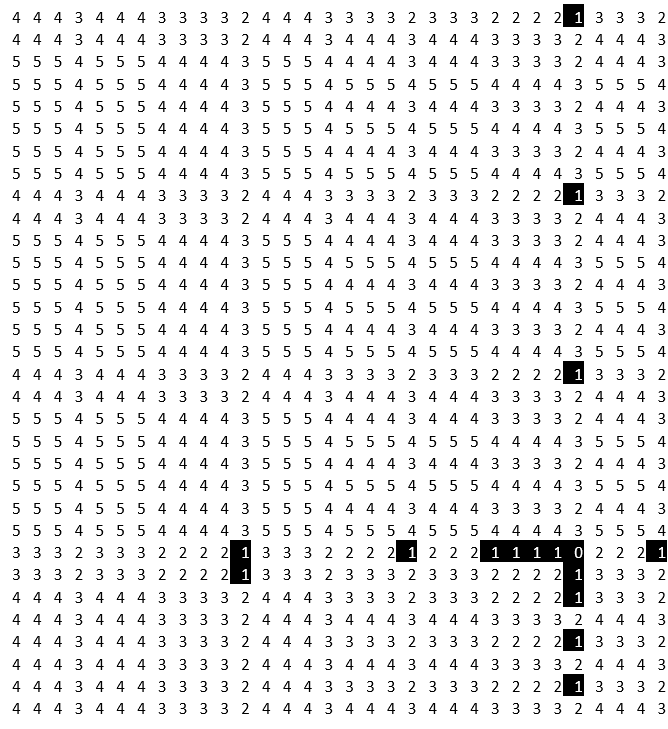
\includegraphics[width=0.95\textwidth]{img/1} $d-d_{y'} = 1$ \end{minipage}% 
				\begin{minipage}{.33\textwidth} \centering 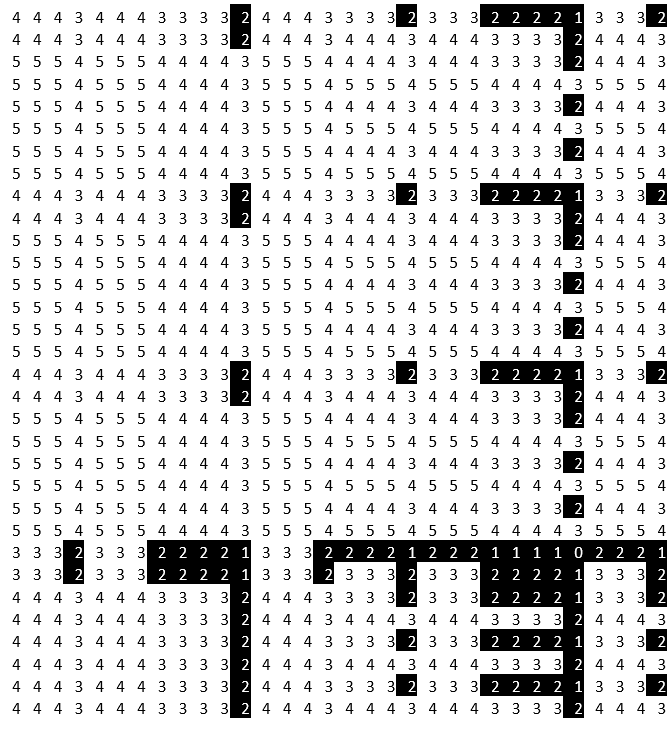
\includegraphics[width=0.95\textwidth]{img/2} $d-d_{y'} = 2$ \end{minipage}
				\newline\vspace*{20pt}\newline
				\begin{minipage}{.33\textwidth} \centering 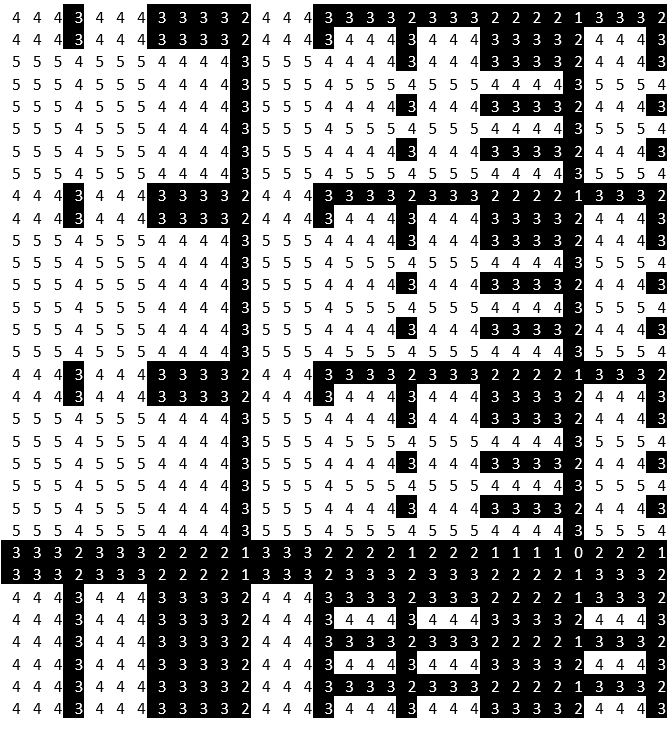
\includegraphics[width=0.95\textwidth]{img/3} $d-d_{y'} = 3$ \end{minipage}%
				\begin{minipage}{.33\textwidth} \centering 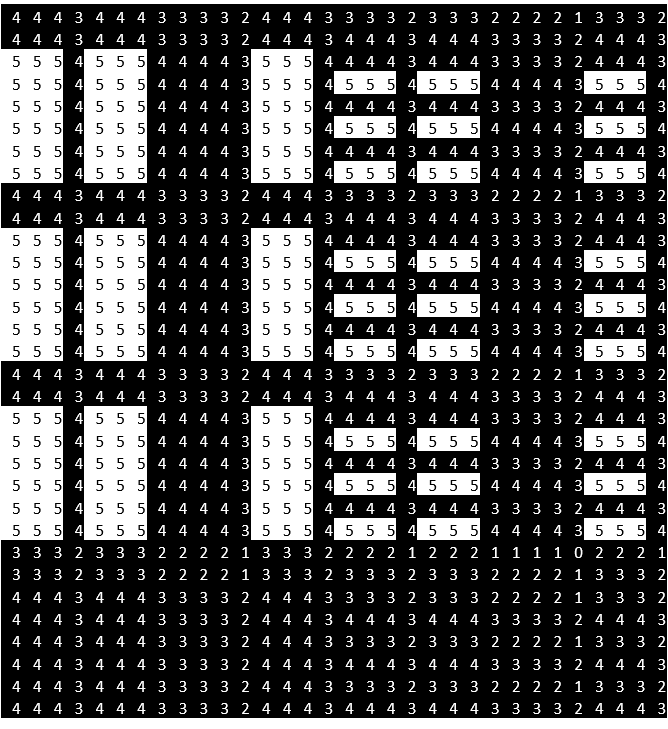
\includegraphics[width=0.95\textwidth]{img/4} $d-d_{y'} = 4$ \end{minipage}%
				\begin{minipage}{.33\textwidth} \centering 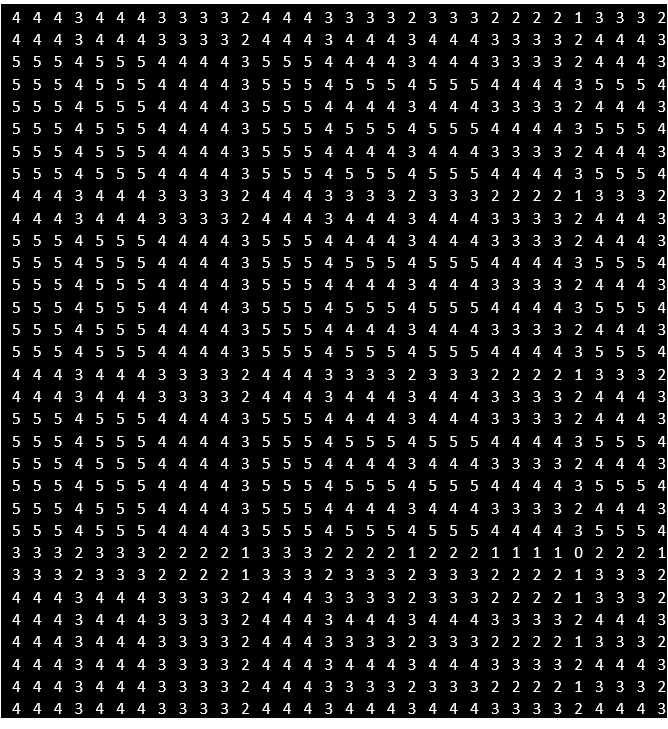
\includegraphics[width=0.95\textwidth]{img/5} $d-d_{y'} \geq 5$ \end{minipage}
				\newline\newline
				\caption{
					Bit patterns followed by blocks in $N(\texttt{tacgt}, 5)$. Black signifies a bit set to 1. There are (5 + 2) = 7 possible patterns; the ``empty'' pattern (for $d - d_{y'} \leq 0$, in which all bits are 0) is not shown. Compare the structure of these patterns with the coloring of the distribution $D(\texttt{tacgt})$ in Figure 4.\ref{fig:D_tacgt}.
					}
			\end{figure}

		\begin{enumerate}
			\setcounter{enumi}{\theenumTemp}
			
			\item There are $4^k$ possible sets of ($k+2$) patterns, one set for each possible ``center'' $k$-suffix in the block. To generate all such sets of patterns, we use Algorithm 4.1.

			\bigskip\bigskip

			{
			\setstretch{1.0}
			\noindent \hspace*{6pt}{\bf Algorithm 4.1}
			\textsc{Block Pattern Generation}\small
			\begin{algorithmic}[1]\label{alg:block-pattern-gen}
				\Require block degree $k$
				\Ensure 3D bit-array $\mathcal{P}$ containing all possible non-trivial block patterns \vspace*{6pt}

				\State $\mathcal{P}[][][] \leftarrow \{\}$ \hspace*{90pt}
				\Comment{retrieve a pattern $P$ as $\mathcal{P}[z][d - d_{y'}]$ }

				\For {$z \leftarrow 0$ to $4^k$}
				\For {$j \leftarrow 1$ to $k-1$}
				\For {$z' \leftarrow 0$ to $4^k$}
				\If{$dH(z,z') \leq j$} 
					\State $\mathcal{P}[z][j][z'] \leftarrow 1$
				\Else
					\State $\mathcal{P}[z][j][z'] \leftarrow 0$
				\EndIf\EndFor\EndFor\EndFor
				\State\Return $\mathcal{P}$
				\end{algorithmic}
			}
			\bigskip
			\noindent After generating $\mathcal{P}$, we can retrieve the set of patterns centered at any $k$-suffix $z$ as $\mathcal{P}[z] = \{P_{1},...,P_{k-1}\}$. These can be used as bit-masks for blocks in the neighborhood bit-array of any $l$-mer $x$ ending in $z$. Notice that the set $\mathcal{P}[z]$ does not include the empty pattern $P_{-1}$ (all 0's), the full pattern $P_{k}$ (all 1's), and the pattern $P_{0}$ in which only the center bit (the bit at position $z$) is set. This is to save space: since applying these patterns to blocks is trivial and does not require block masking, we need not generate and store them in $\mathcal{P}$.
		\end{enumerate}

	\newpage
	\section{Implementing a pattern-based speedup technique for EMS-GT}
		The previous section has shown that the bit-array $N$, representing the $d$-neighborhood of an $l$-mer, can be defined in terms of repeating block patterns. This definition can be used toward a larger goal---constructing the bit-array $\mathcal{N}$ which represents the $d$-neighborhood $\mathcal{N}(S,d)$ of a sequence $S$.

		To do this, we first initialize the array $\mathcal{N}$ of $4^l$ bit flags, all set to zero. We select a value for the block degree $k$, and pre-generate all $4^k$ possible sets of block patterns (using Algorithm 4.1). Then, for every $l$-mer $x = yz$ in $S$:
		\begin{enumerate}
			\item We retrieve $\mathcal{P}(z) = \{P_{1}, ... , P_{k-1}\}$, the set of unique block patterns ``centered'' at $x$'s $k$-suffix $z$. For convenience, this set excludes three ``trivial'' patterns: the empty pattern $P_{-1}$ (all 0's), the full pattern $P_{k}$ (all 1's), and the pattern $P_{0}$ in which only the center bit (the bit at position $z$) is set.
			\item For every $d$-neighbor $y'$ of $x$'s prefix $y$, we locate the block---$block(\mathcal{N}, y')$---in $\mathcal{N}$ whose block prefix is $y'$. We then apply the appropriate pattern to the block, based on the value of $d - d_{y'}$:
			\begin{enumerate}
				\item If $d - d_{y'} = 0$, we set the ``center'' bit, i.e. the bit at position $z$ in $block(\mathcal{N}, y')$.
				\item If $0 < d - d_{y'} < k$, we mask the pattern $P_{d - d_{y'}}$ onto $block(\mathcal{N}, y')$.
				% This means that, for every bit set to 1 in the pattern, the corresponding bit of $block(\mathcal{N}, y')$ will also be set.
				\item If $d - d_{y'} \geq k$, we set all bits in $block(\mathcal{N}, y')$.
			\end{enumerate}
			% This traverses and masks all non-empty blocks---those which fulfill the condition $d - d_{y'} \geq 0$; in other words, those for which the block prefix $y'$ is a neighbor of $y$.
		\end{enumerate}

		\noindent This entire procedure effectively performs $\mathcal{N}(S,d) \leftarrow \mathcal{N}(S,d) \cup N(x,d)$ for each $l$-mer $x$ in $S$, as specified in lines 3-6 and 10-13 of EMS-GT (Algorithm 2.1).

	\section{Performance improvement with pattern-based speedup technique}
		The pattern-based technique requires examining all $d$-neighbors of $x$'s prefix $y$.
		We can use our recursive procedure (Algorithm 2.3) to traverse the neighborhood $N(y,d)$; as Table \ref{tbl:neighbors_blockmasking} shows, this will require generating much fewer neighbors than $N(x,d)$:\newline

		\begin{table}[h] %neighbors_blockmasking
			\small
			\renewcommand{\arraystretch}{1.3}
			\label{tbl:neighbors_blockmasking}
			\centering
			\begin{tabular}{|c|c|c|c|}
			\hline 
			\bfseries\boldmath $(l,d)$ & \bfseries\boldmath $N(x,d)$ & \bfseries\boldmath $N(y,d)$, $k$=5 & \bfseries \% reduction\\
			\bfseries & \bfseries\boldmath $\sum_{i=0}^{d} \binom{l}{i} 3^{i}$ & \bfseries\boldmath $\sum_{i=0}^{d} \binom{l-k}{i} 3^{i}$ & \\
			\hline
			 9,2 &         351  &       66 & 81.2\%\\
			11,3 &       4,983  &      693 & 86.1\%\\
			13,4 &      66,378  &    7,458 & 88.8\%\\
			% 14,4 &      91,770  &   12,825 & 86.0\%\\
			15,5 &     853,569  &   81,921 & 90.4\%\\
			% 16,5 &   1,225,092  &  143,979 & 88.2\%\\
			17,6 &  10,738,203  &  912,717 & 91.5\%\\
			\hline\end{tabular}

			\caption{\small Number of individual neighbors generated for $N(x,d)$ vs. $N(y,d)$}
			\end{table}

		\noindent This large reduction in neighbors generated partly explains why, for most $(l,d)$ values, building the neighborhood in blocks proves significantly faster (Table 4.\ref{tbl:speedup_blockmasking}) than recursively generating each individual neighbor, then locating and setting its bit flag. \newline 

		\begin{table}[h] %speedup_blockmasking
			\small
			\renewcommand{\arraystretch}{1.3}
			\label{tbl:speedup_blockmasking}
			\centering
			\begin{tabular}{|c|c|c|c|}
			\hline 
			\bfseries\boldmath $(l,d)$ & \bfseries Without pattern-based & \bfseries With pattern-based & \bfseries speedup\\
			\bfseries & \bfseries procedure & \bfseries\boldmath procedure, $k=5$ & \bfseries\\
			\hline
			 9,2 &   0.06 s &    0.11 s &     --  \\
			11,3 &   0.22 s &    0.20 s &    6.7\%\\
			13,4 &   1.98 s &    1.04 s &   47.5\%\\
			% 14,4 &   3.53 s &    2.55 s &   27.8\%\\
			15,5 &  25.06 s &   15.51 s &   38.1\%\\
			% 16,5 &  41.63 s &   29.03 s &   30.3\%\\
			17,6 & 308.61 s &  175.85 s &   43.0\%\\
			\hline\end{tabular}

			\caption{\small Performance of EMS-GT with vs. without pattern-based speedup
			(runtimes averaged over 20 synthetic datasets for each $(l,d)$ instance).}
			\end{table}

		\subsection{Determining the optimum block size}
			In the previous sections on distance-based patterns, the block degree $k$ was set to 5, thus the size of blocks in $N$ was $4^5 = 32 \times 32$. Based on empirical results in Table 4.\ref{tbl:block-degree-tests},\ \ $k=5$ is in fact an optimal value for solving the $(l,d)$ challenge instances used for evaluation:\newline

			\begin{table}[h] %block-degree-tests
				\small
				\renewcommand{\arraystretch}{1.3}
				\label{tbl:block-degree-tests}
				\centering
				\begin{tabular}{|c|c|c|c|c|c|}
				\hline
				\bfseries\boldmath $(l,d)$ &
				\bfseries\boldmath $k=3$ &
				\bfseries\boldmath $k=4$ &
				\bfseries\boldmath $k=5$ &
				\bfseries\boldmath $k=6$ &
				\bfseries\boldmath $k=7$ \\

				\bfseries &
				\bfseries\boldmath $32 \times   2$ blk &
				\bfseries\boldmath $32 \times   8$ blk &
				\bfseries\boldmath $32 \times  32$ blk &
				\bfseries\boldmath $32 \times 128$ blk &
				\bfseries\boldmath $32 \times 512$ blk \\
				\hline
				 9,2 	&    -   &    -     & {\bf  0.11 s} &  0.57 s &  9.02 s \\
				11,3 	&    -   &    -     & {\bf  0.20 s} &  0.70 s &  9.77 s \\
				13,4 	&  1.74 s &  1.31 s & {\bf  1.04 s} &  2.19 s & 12.40 s \\
				15,5 	& 23.43 s & 21.43 s & {\bf 15.51 s} & 24.28 s & 46.30 s \\
				% 17,6 	&	&	&	&	&\\
				\hline
				\end{tabular}
				\centering
				\caption{\small Performance of EMS-GT (with pattern-based speedup) for different values of $k$. Shortest times are in bold text.}
				\end{table}

			% Insight for why k=5 is optimal
			% It appears $k=5$ allows for the best balance of block size and number of patterns.
			When $k$ is lower, there are fewer and smaller block patterns to manage, but building $N$ requires many highly scattered array accesses to small blocks. When $k$ is higher, there are larger contiguous blocks and thus fewer accesses in $N$, but also a much larger set of block patterns to manage. It seems that $k=5$ allows for the most efficient balance between recursive neighbor generation (which identifies and accesses blocks according to their prefixes) and bit-masking operations (which selects and applies the correct pattern to each block), with a feasible number of block patterns. 

	\section{Performance of improved EMS-GT}
		Finally, the improved EMS-GT and two competitor algorithms were run on an Intel Xeon, 2.10 GHz processor (single core only). Their performance, averaged over 20 synthetic datasets for each $(l,d)$ challenge instance, is outlined in Table 4.\ref{tbl:runtimes_v_pms}:\newline

		\begin{table}[ht] %runtimes
			\small
			\renewcommand{\arraystretch}{1.3}
			\label{tbl:runtimes_v_pms}
			\centering
			\begin{tabular}{|c|c|c|c|c|}
			\hline \bfseries\boldmath $(l,d)$ & \bfseries PMS8 & \bfseries qPMS9 & \bfseries EMS-GT & \bfseries \% speedup\\
			\hline
			 9,2 &  0.74 s  &  0.47 s & {\bf 0.11 s} & 76.6\%\\
			11,3 &  1.58 s  &  1.06 s & {\bf 0.20 s} & 81.1\%\\
			13,4 &  5.39 s  &  4.52 s & {\bf 1.04 s} & 77.0\%\\
			% 14,4 &  1.29 s  &  1.02 s &      2.55 s\\
			15,5 & 36.45 s  & 24.63 s & {\bf15.51 s} & 37.0\%\\
			% 16,5 &  4.79 s  &  2.96 s &     29.03 s\\
			17,6 &  3.91 min & \textbf{1.96 min} & {\emph{2.93 min}} & --\\
			\hline\end{tabular}

			\caption{\small Runtimes of PMS8, qPMS9 and EMS-GT. Shortest times are in bold text.}
			\end{table}

		For every challenge instance except (17,6) the improved EMS-GT outperforms qPMS9; it outperforms PMS8 for (17,6). EMS-GT was run including the pattern-based speedup technique, with the default suffix length of $k=5$. Observe that EMS-GT can only solve problem instances where $l \leq 17$. This is because when we reach $l$=18, the size of the integer array needed to represent the entire search space ($\frac{4^{18}}{32} = \frac{2^{36}}{2^{5}} = 2^{31}$ integers) begins to exceed the maximum size for Java arrays, which is ($2^{31} - 1$) elements.\newline

		\begin{table}[ht] %runtimes
			\small
			\renewcommand{\arraystretch}{1.3}
			\label{tbl:runtimes_nonchallenge}
			\centering
			\begin{tabular}{|c|c|c|c|}
			\hline \bfseries\boldmath $(l,d)$ & \bfseries PMS8 & \bfseries qPMS9 & \bfseries EMS-GT \\
			\hline
			14,4 &  1.29 s  &  1.02 s &      2.55 s\\
			16,5 &  4.79 s  &  2.96 s &     29.03 s\\
			\hline\end{tabular}

			\caption{\small Performance of PMS8, qPMS9 and EMS-GT on non-challenging ($l$,$d$).}
			\end{table}

		EMS-GT is highly competitive with PMS8 and qPMS9 on challenging problem instances, but as Table 4.\ref{tbl:runtimes_nonchallenge} shows, on non-challenging instances EMS-GT is not as efficient. This may be due to differing representations of the search space: while EMS-GT uses a fixed-size bit-array to represent the search space of all $4^l$ $l$-mers, PMS8 and qPMS9 have a dynamically-sized search space which, while easily managed for most ($l$,$d$) values, may be more inefficient to narrow down for challenging ($l$,$d$) values.

\chapter{Conclusion}
	This paper discusses a novel speedup technique for the EMS-GT algorithm, an exact solution to the planted motif problem. A Java implementation, run on various challenge problem instances, shows the improved algorithm to be very competitive against state-of-the-art exact algorithms PMS8 and qPMS9. The speedup technique allows EMS-GT to outperform the current best algorithm, qPMS9, for the challenge problem instances (9,2), (11,3), (13,4) and (15,5) with a run-time reduction of at least 76\%, 81\%, 77\% and 37\% respectively for these instances, while ranking second to qPMS9 for test instance (17,6). 

	Directions for further research include: refining the bit-based storage mechanism to be able to represent the entire motif search space for $l > 17$; creating a multiprocessor version of EMS-GT to solve in parallel for larger values of ($l$,$d$); and delegating the bit-masking optimization and other bulk bit operations to the graphics card, as explored in \cite{dasari2010efficient}, for faster performance.

\BackMatter
\bibliographystyle{plain}
\bibliography{sources}
%\addappheadtotoc
%\input{APPENDIX}

\end{document}
